\subsection{Photo-multipliers surface coating}

\paragraph{p-terphenyl recoating}


\begin{figure}[h]
	\centering
	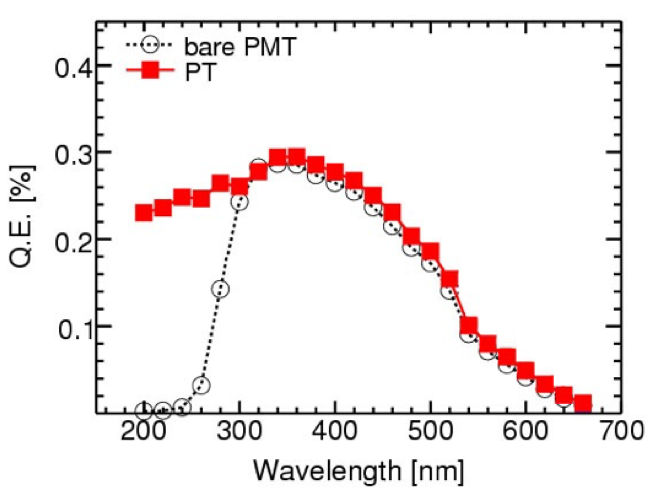
\includegraphics[width=1.0\columnwidth,keepaspectratio]{img/pmtQuantumEfficiencyGain.png}
	\caption{Average number of reflections calculated from simulations studies.}
	\label{fig:pmtQuantumEfficiencyGain}
\end{figure}

\begin{figure}[h]
	\centering
	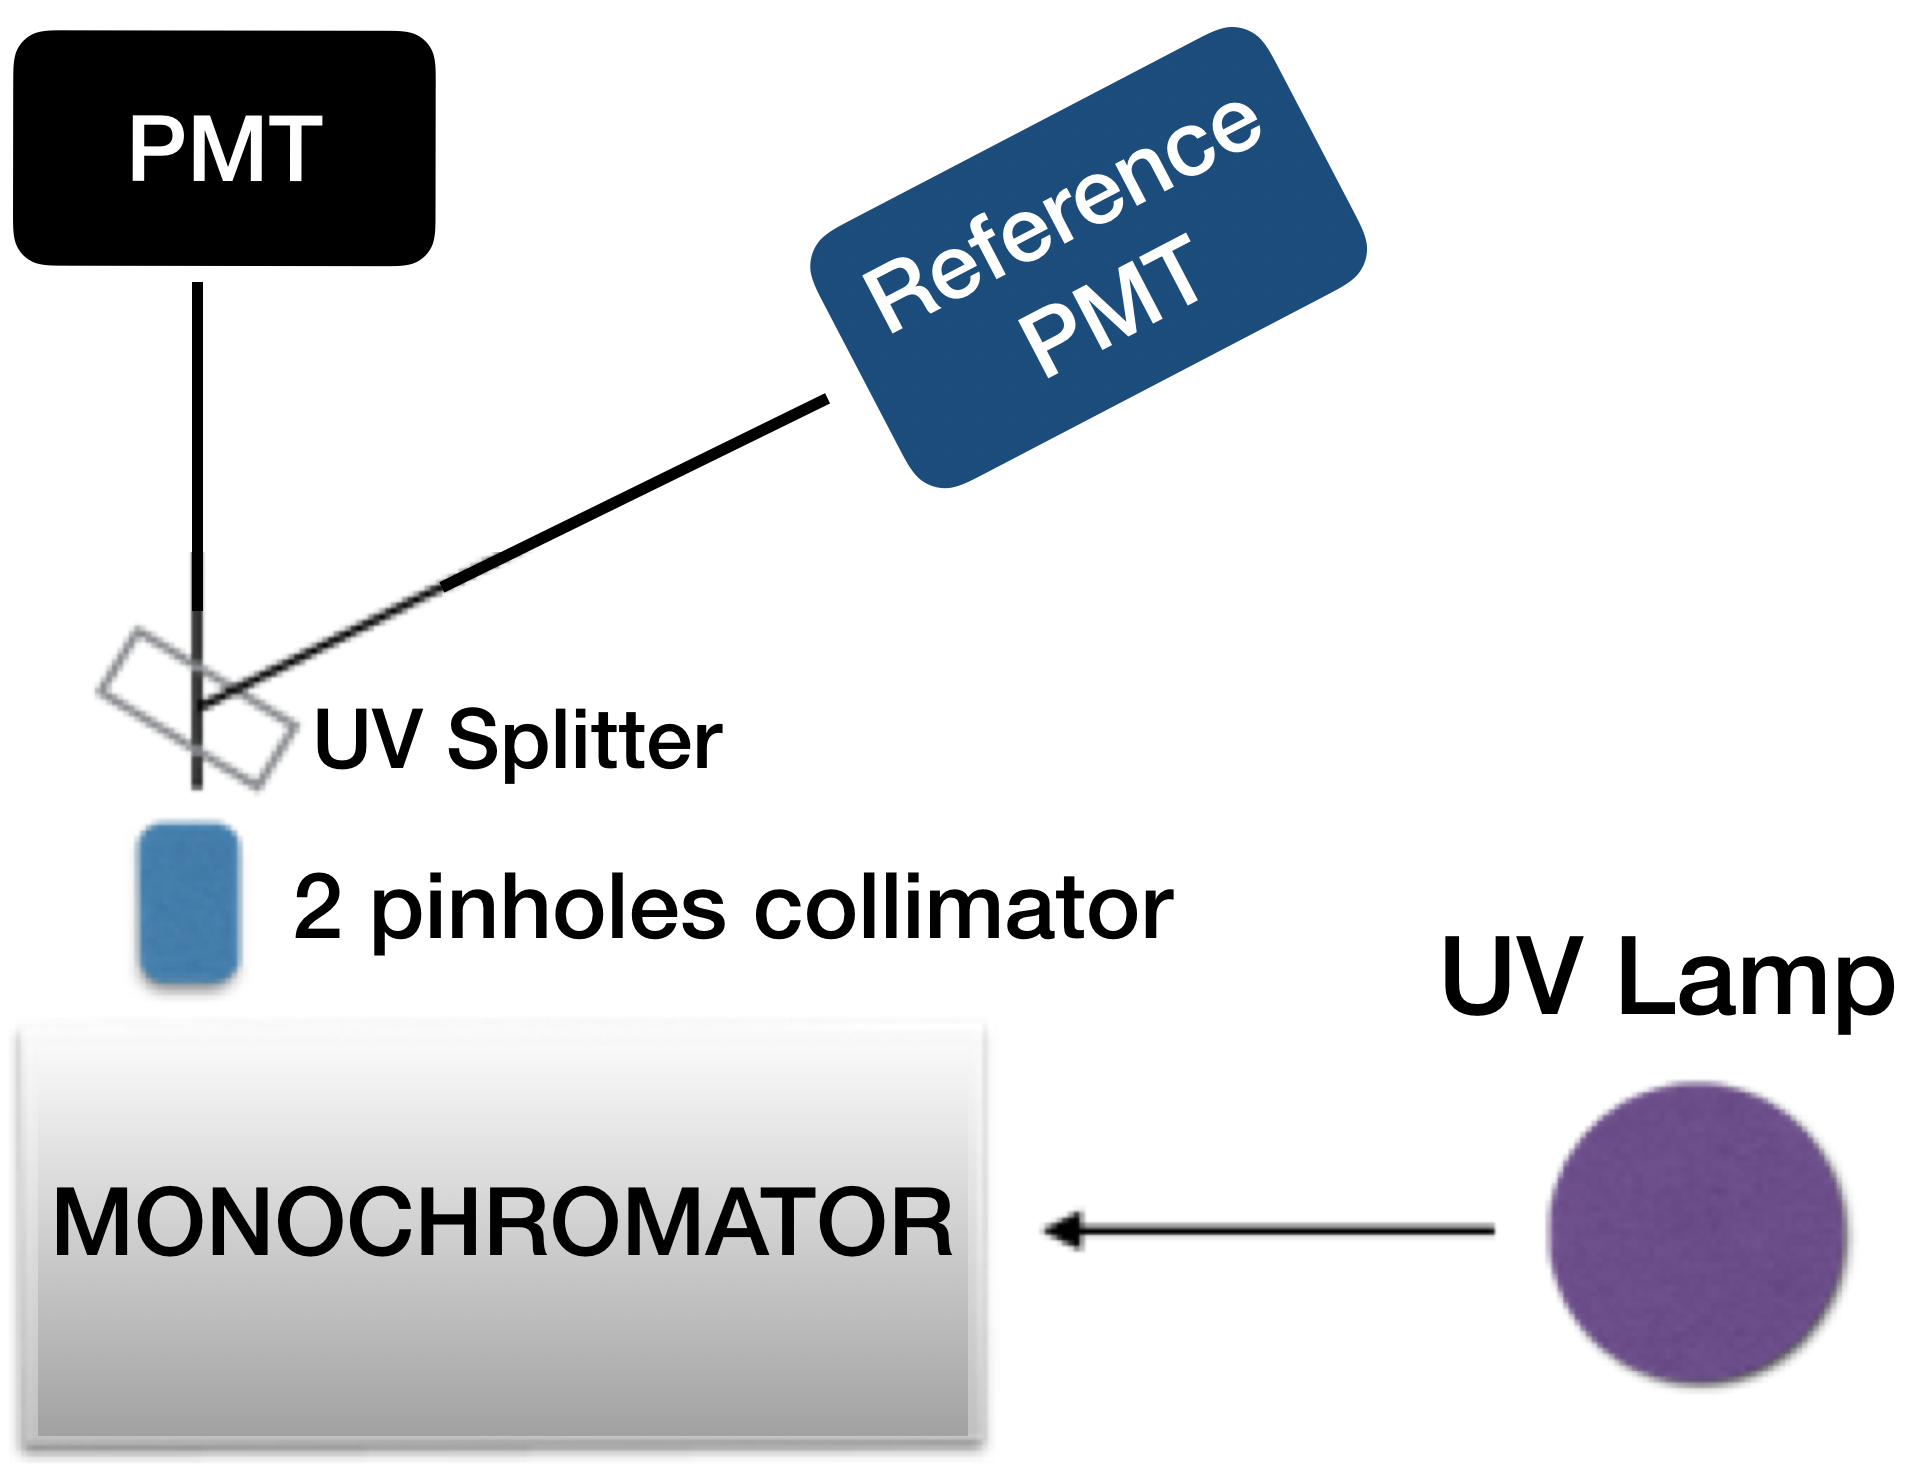
\includegraphics[width=1.0\columnwidth,keepaspectratio]{img/pmtTestingSetup.png}
	\caption{Average number of reflections calculated from simulations studies.}
	\label{fig:pmtTestingSetup}
\end{figure}





\paragraph{base modification: 2 x10 output}

\begin{figure}[h]
	\centering
	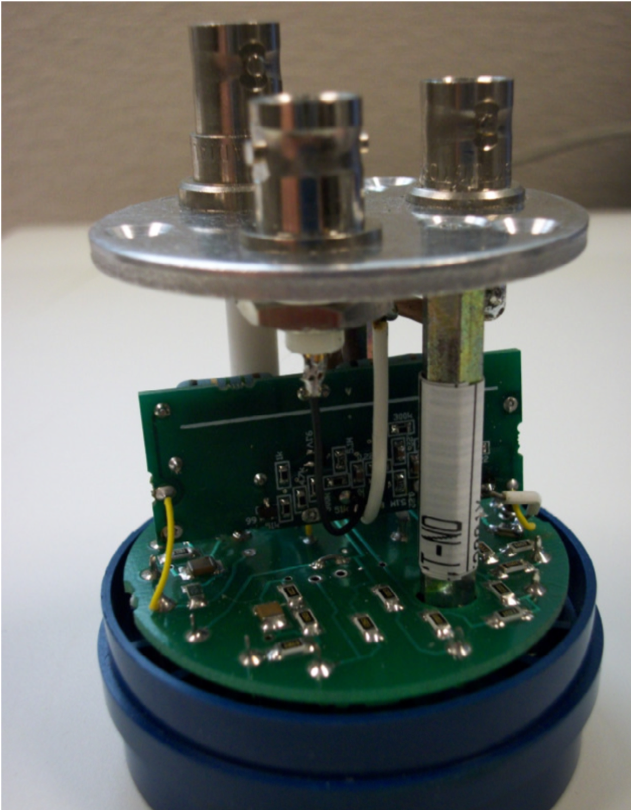
\includegraphics[width=1.0\columnwidth,keepaspectratio]{img/pmtWithDivider.png}
	\caption{Average number of reflections calculated from simulations studies.}
	\label{fig:pmtWithDivider}
\end{figure}
